Para el análisis de los gráficos se añadió una curva del comportamiento teórico para poder comparar el comportamiento de los datos recogídos, divididos en el tipo de grilla, y dominio según si era necesario.
Para contrastar las mediciones con la complejidad teórica, los gráficos de tiempo y memoria incluyen la curva teórica de cada algoritmo escalada por un factor $c$. Como la cota asintótica describe el crecimiento salvo una constante, $c$ se calibra mediante mínimos cuadrados en escala logarítmica sobre las grillas libres, que no admiten podas, de modo que la comparación se hace sobre la forma de la curva y no sobre su magnitud absoluta.

\subsection {Paradigmas de diseño de algoritmos}

\subsubsection {Fuerza Bruta}
El paradigma de fuerza bruta, consiste en enumerar todas las soluciones candidatas y conservar la mejor. Para este problema se implementa una recursión que parte desde $(1, 1)$ y, en cada celda, explora los movimientos de R y D acumulando el puntaje y las vidas restantes, registrando el camino de mayor puntaje al llegar a $(N, M)$. Una rama solo se descarta cuando pisa una muralla o agota las vidas, sin cotas sobre el puntaje ni memorización. En el peor caso recorre los $\binom{N + M - 2}{N - 1}$ caminos posibles, por lo que su tiempo es $O(\binom{N + M - 2}{N - 1})$. Su memoria en cambio, es sólo $O(N + M)$: la profundidad de la recursión y el camino en construcción. \cite {peroni_bruteforce, programmingalgorithms_bf}

Los datos obtenidos se ven representados en estos gráficos:

\begin{figure}[H]
    \centering
    \begin{minipage}{0.48\textwidth}
        \centering
        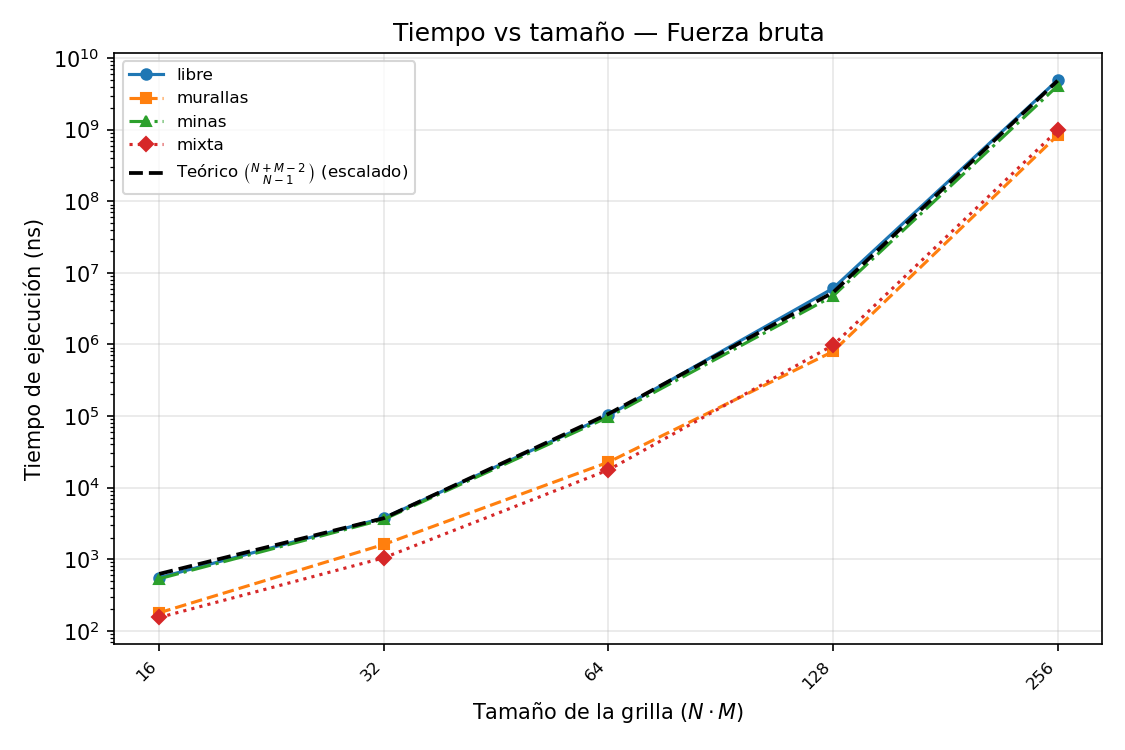
\includegraphics[width=\textwidth, height=4cm, keepaspectratio]{../code/grid_pathfinding/data/plots/time_bruteforce.png}
        \par\vspace{0.2cm}
        \small a) Tiempo de ejecución
    \end{minipage}\hfill
    \begin{minipage}{0.48\textwidth}
        \centering
        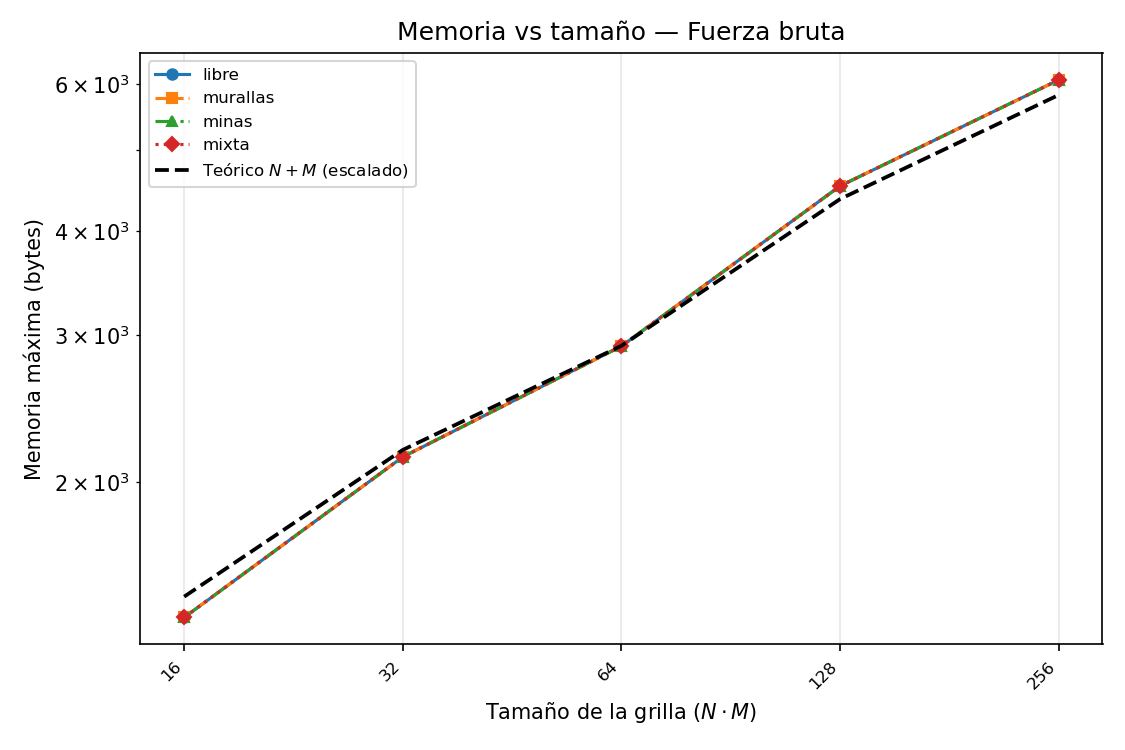
\includegraphics[width=\textwidth, height=4cm, keepaspectratio]{../code/grid_pathfinding/data/plots/mem_bruteforce.png}
        \par\vspace{0.2cm}
        \small b) Consumo de memoria
    \end{minipage}

    \caption{Paradigma Fuerza Bruta - Tiempo de ejecucion (a) y memoria (b) vs. tamaño de la grilla.}
    \label{fig:bruteforce}
\end{figure}

El el gráfico de tiempo se observa que las curvas empíricas de los cuatro tipo de grillas siguen a la curva teórica $\binom{N + M - 2}{N + M}$ con la misma pendiente y curvatura en todos los tamaños. Se vuelven más empinadas al aumentar el tamaño de la grilla, en lugar de crecer de forma recta, lo que es característico del crecimiento exponencial en $N + M$.

En el gráfico de memoria las curvas empíricas crecen de forma lineal y siguen a la curva teórica $O(N + M)$, lo que confirma que el consumo de memoria es muy bajo comparado con el tiempo. Esto se debe a que la recursión no almacena resultados intermedios, lo único que se mantiene es la pila de llamadas, cuya profundidad máxima es proporcional al largo del camino, y la cadena con el camino en construcción. El pico de memoria depende sólo de la profundidad máxima de la recursión.

\subsubsection {Programación Dinámica}
El paradigma de programación dinámica resuelve el problema combimando soluciones óptimas de subproblemas más pequeños, aprovechando su subestructura óptima y almacenando los resultados para no recalcularlos. En este caso, se reconstruye el camino óptimo desde la meta utilizando un enfoque bottom-up. Como cada uno de los $NMV$ estados se resuelve en tiempo constante, tanto el tiempo como la memoria son $O(NMV)$ \cite {cpalgorithms_dp, geeks_tabulation}

Los datos obtenidos se ven representados en estos gráficos:

\begin{figure}[H]
    \centering
    \begin{minipage}{0.48\textwidth}
        \centering
        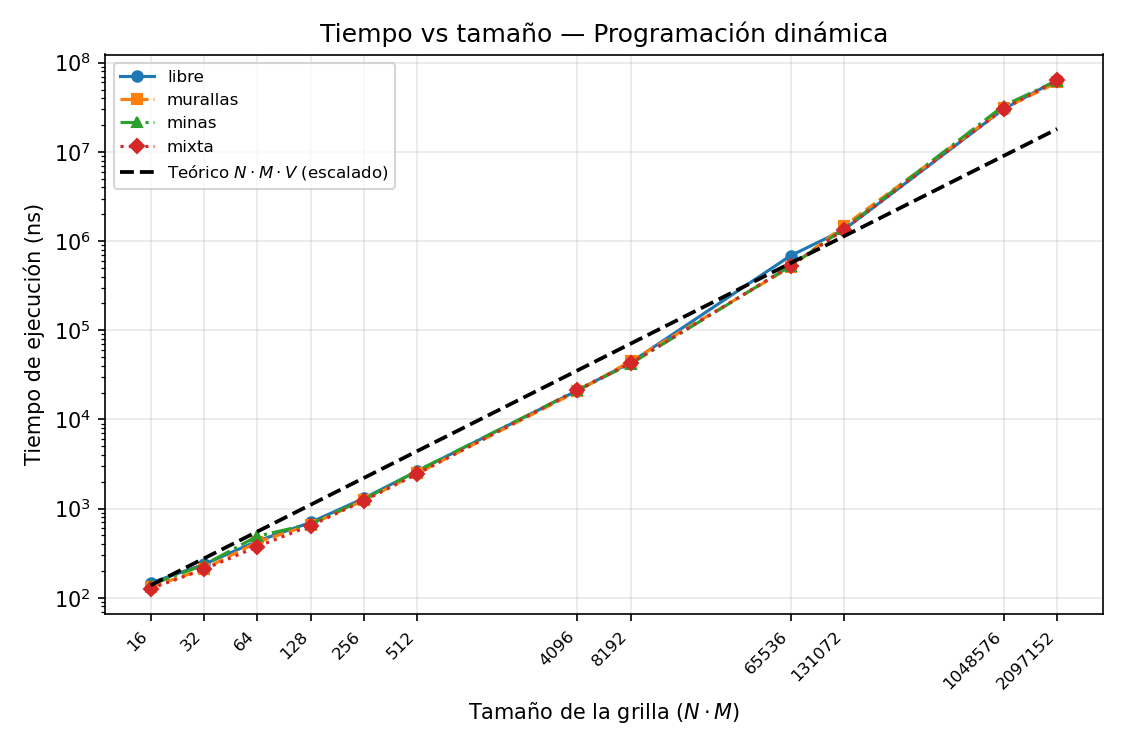
\includegraphics[width=\textwidth, height=4cm, keepaspectratio]{../code/grid_pathfinding/data/plots/time_dp.png}
        \par\vspace{0.2cm}
        \small a) Tiempo de ejecución
    \end{minipage}\hfill
    \begin{minipage}{0.48\textwidth}
        \centering
        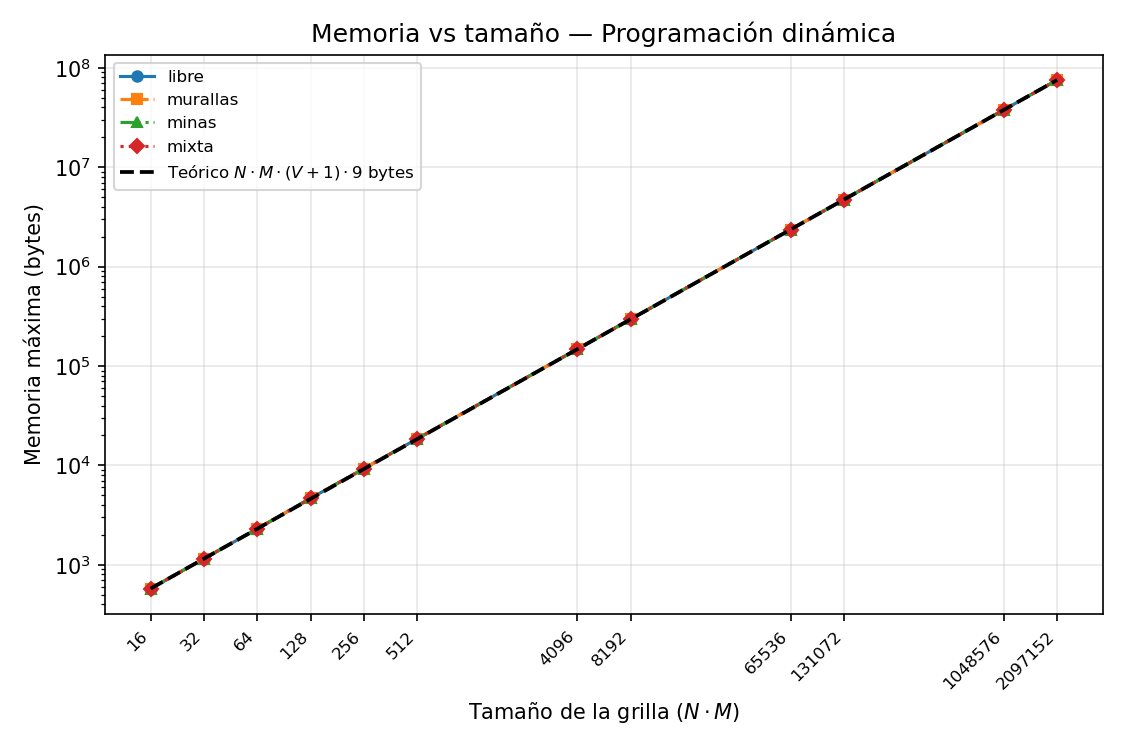
\includegraphics[width=\textwidth, height=4cm, keepaspectratio]{../code/grid_pathfinding/data/plots/mem_dp.png}
        \par\vspace{0.2cm}
        \small b) Consumo de memoria
    \end{minipage}

    \caption{Paradigma Programación Dinámica - Tiempo de ejecucion (a) y memoria (b) vs. tamaño de la grilla.}
    \label{fig:dp}
\end{figure}

En el gráfico de tiempo las curvas de los cuatro tipos de grilla prácticamente coinciden y siguen a la curva teórica $N\cdot M\cdot V$ con una tendencia lineal en la mayor parte del rango de tamaños. Como $V$ es constante, el tiempo crece de forma proporcional al tamaño de la grilla. Esto se debe a que la implementación calcula cada estado una sola vez, consultando los dos estados predecesores ya resueltos, sin repetir subproblemas, de modoque el trabajo por estado es constante.

En el gráfico de memoria las curvas empíricas coinciden con la teórica $N\cdot M\cdot (V + 1)\cdot 9$ bytes en todos los tamaños. Como esta curva no está escalada, la coincidencia confirma tanto la forma lineal en $N\cdot M$ como la magnitud del consumo. La memoria utilizada corresponde a las dos tablas de la implementación, una de puntaje y otra de procedencia, con un estado por cada celda y cada nivel de vidas. Al depender sólo de las dimensiones de las grillas y de $V$, y no de su contenido, la memoria es idéntica para los cuatro tipos de grillas.

\subsubsection {Greedy}
El paradigma greedy construye el camino tomando en cada celda la decisión localmente más conveniente, sin reconstruirla. Desde la posición actual evalúa los movimientos R y D, descarta las celdas fuera de la grilla, las murallas y las minas cuando queda una sola vida, y avanza hacia la de mayor ganancia neta, prefiriendo la derecha en caso de empate. Realiza a los más $N + M - 2$ pasos de costo constante, por lo que su tiempo es de $O(N + M)$, y su memoria también es de $O(N + M)$ \cite {codecademy_greedy}

Los datos obtenidos se ven representados en estos gráficos:

\begin{figure}[H]
    \centering
    \begin{minipage}{0.48\textwidth}
        \centering
        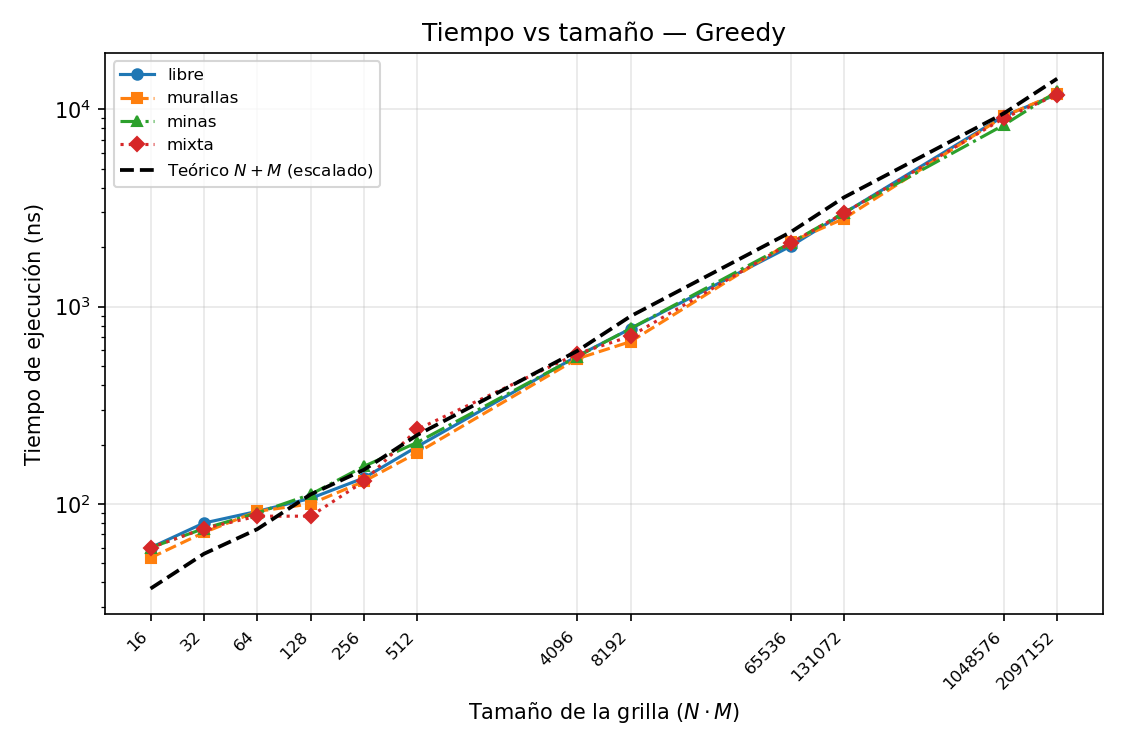
\includegraphics[width=\textwidth, height=4cm, keepaspectratio]{../code/grid_pathfinding/data/plots/time_greedy.png}
        \par\vspace{0.2cm}
        \small a) Tiempo de ejecución
    \end{minipage}\hfill
    \begin{minipage}{0.48\textwidth}
        \centering
        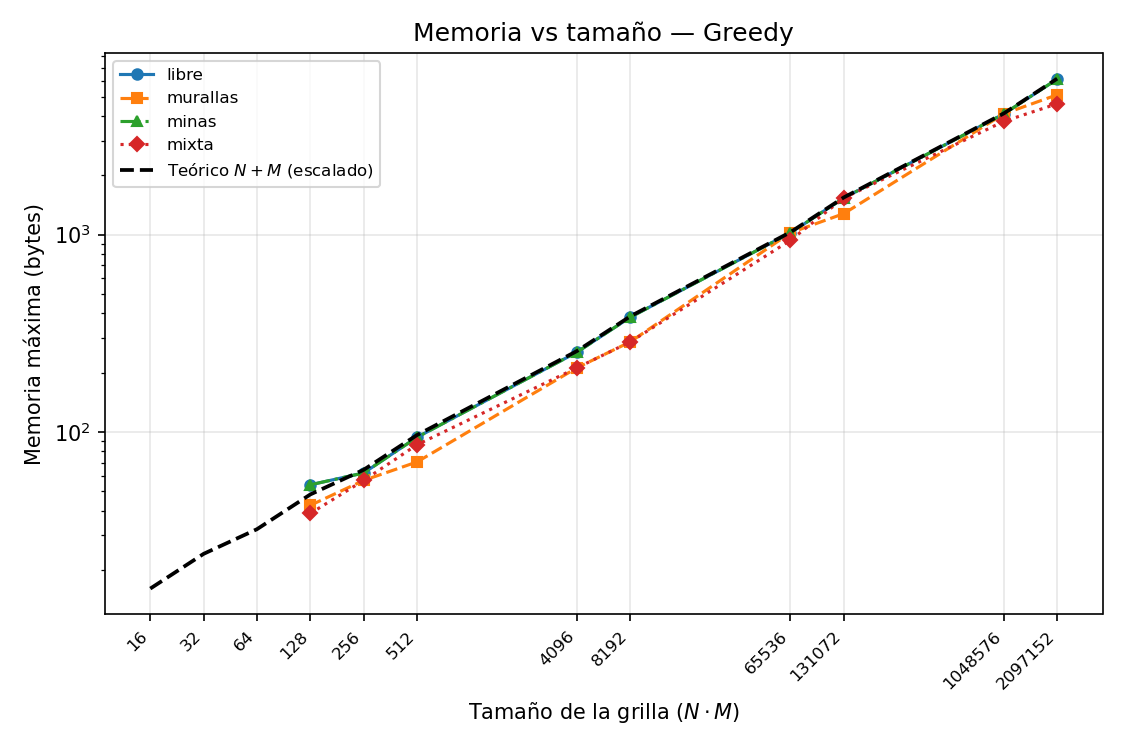
\includegraphics[width=\textwidth, height=4cm, keepaspectratio]{../code/grid_pathfinding/data/plots/mem_greedy.png}
        \par\vspace{0.2cm}
        \small b) Consumo de memoria
    \end{minipage}

    \caption{Paradigma Fuerza Bruta - Tiempo de ejecucion (a) y memoria (b) vs. tamaño de la grilla.}
    \label{fig:greedy}
\end{figure}

En el gráfico de tiempo las curvas experimentales de los cuatro tipos de grilla crecen con la misma tendencia que la curva teórica $N + M$ a lo largo de todo el rango, lo que confirma el comportamiento lineal. Esto se debe a que se recorre el camino una sola vez, de la celda inicial a la meta, y en cada paso sólo compara dos celdas vecinas, de modo que el trabajo depende del largo del camino.

En el gráfico de memoria las curvas crecen con la misma tendencia que la curva teórica $N + M$, lo que confirma el crecimiento lineal. Esto se debe a que el algoritmon no utiliza estructuras auxiliare, lo único que almacena es la cadena con los movimientos del camino.

Los datos obtenidos sobre la brecha se ven representados en estos gráficos:

\begin{figure}[H]
    \centering
    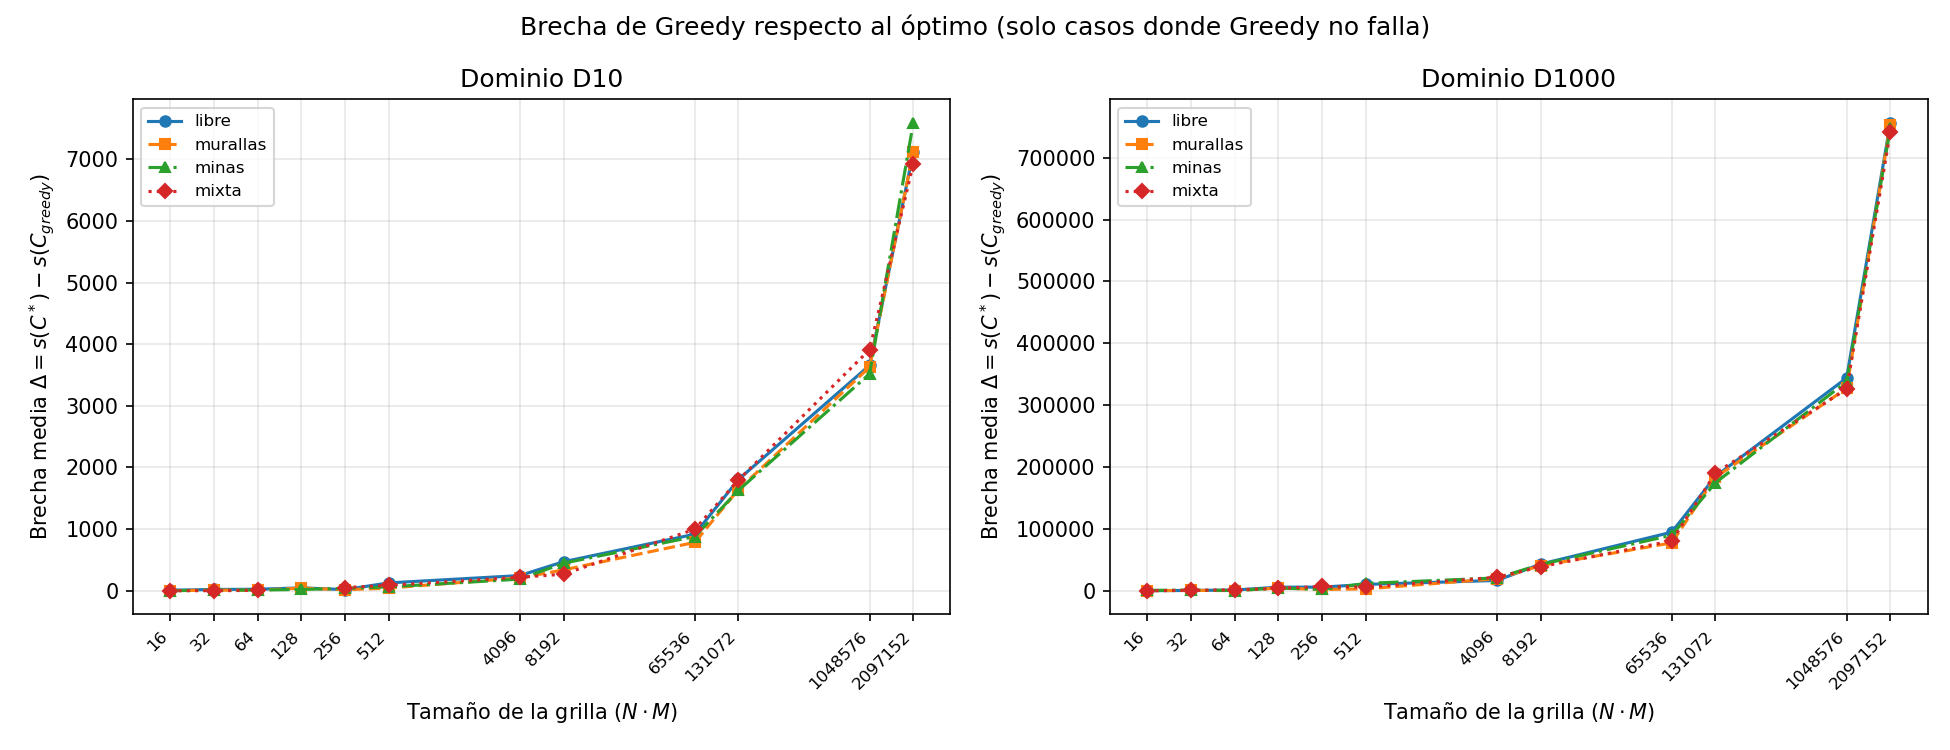
\includegraphics[width=\textwidth, height=4cm, keepaspectratio]{../code/grid_pathfinding/data/plots/gap_vs_size.png}
    \caption{Brecha: Comparación soluciones óptimas de Greedy vs DP, según el dominio de la grilla.}
    \label{fig:gap}
\end{figure}

En el gráfico de la brecha, que considera sólo los casos en que greedy encuentra un camino, se observa que la diferencia entre la solución óptimay la de greedy es muy pequeña en las grillas pequeñas y crece de forma sostenida con el tamaño de la grilla. Esto se debe a que greedy decide sólo con la información de la vecina inmediata, y mientras más largo es el camino, las decisiones que toma lo alejan del óptimo. En las grillas pequeñas, con pocas decisiones, suele coincidir con el óptimo.

Los datos obtenidos sobre la tasa de fallos se ven representados en estos gráficos:

\begin{figure}[H]
    \centering
    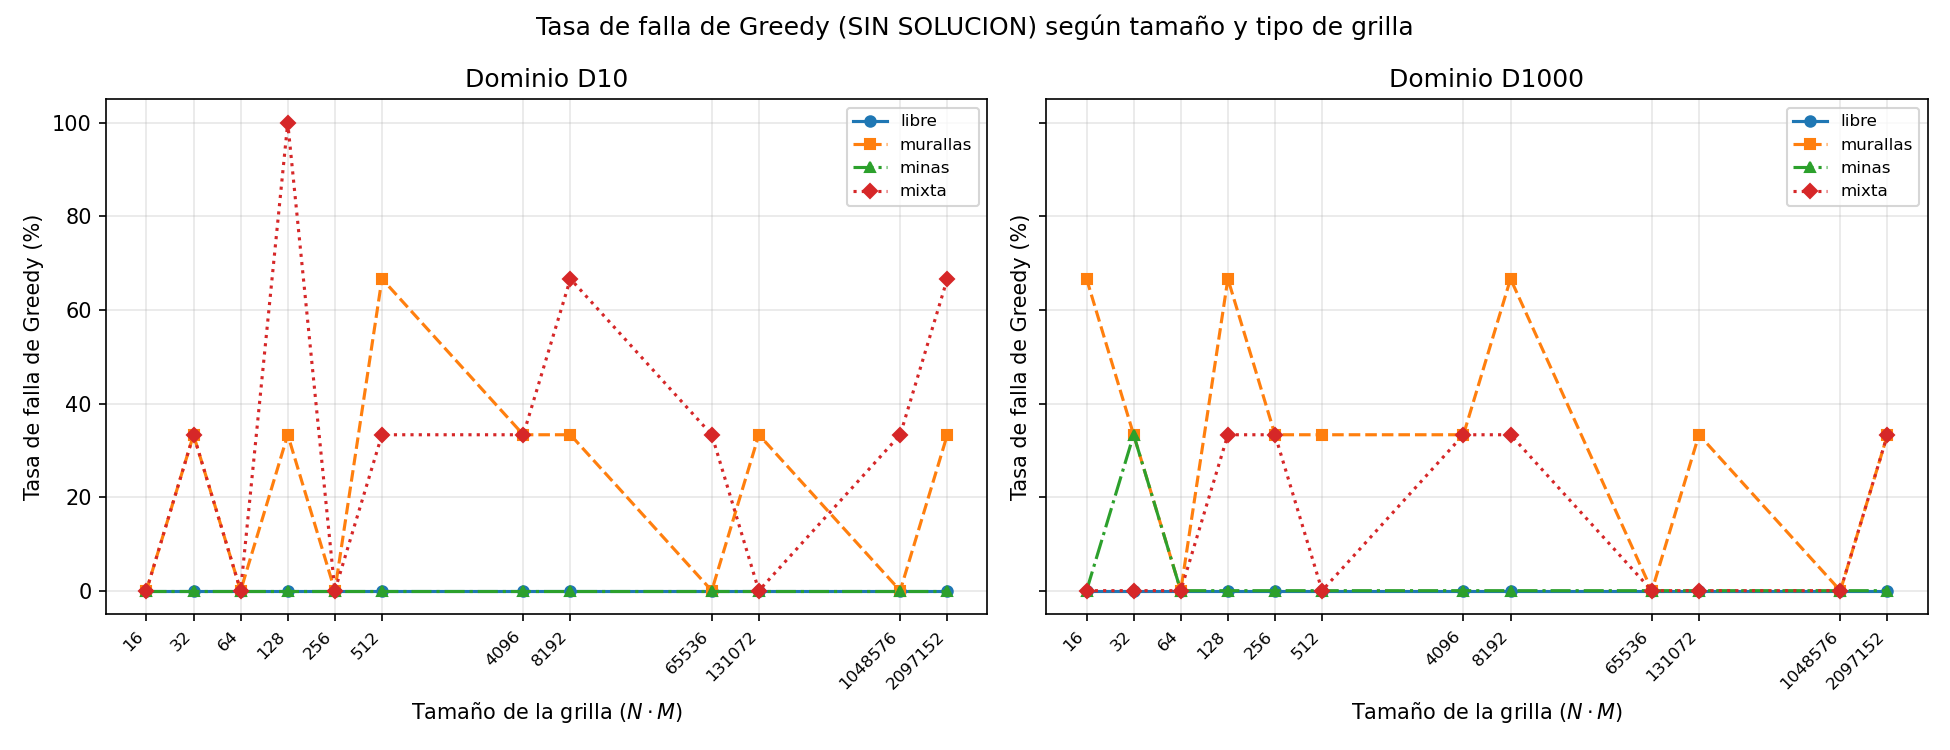
\includegraphics[width=\textwidth, height=4cm, keepaspectratio]{../code/grid_pathfinding/data/plots/failure_rate_vs_size.png}
    \caption{Tasa de fallo de greedy vs dominio de la grilla.}
    \label{fig:failure}
\end{figure}

En el gráfico de la tasa de falla se observa que greedy no falla en las grillas libres y casi nunca en las de minas, mientras que en las grillas con murallas falla con frecuencia, sin una tendencia clara respecto del tamaño. Esto se debe a que sin murallas, siempre hay al menos una vecina transitable, y las minas sólo bloquean al algoritmo cuando queda una sola vida y no existe otra opción. Como no se puede retroceder ni reconsiderar una decisión, queda atrapado en un callejón sin salida aunque exista un camino válido.

\textbf{Repositorio con la data utilizada:} \url{https://github.com/majozZzz/Tarea2-INF221.git}
